\begin{figure}[t]
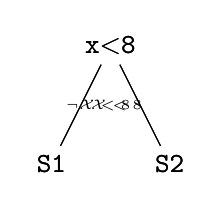
\begin{tikzpicture}[]
  \node {\texttt{x$<$8}}
     child {
        node[xshift=0mm, yshift=0mm] {\texttt{S1}}
        edge from parent
        node[right] {\tiny ${\cal X} < 8$}
     }
     child {
        node[xshift=0mm, yshift=0mm] {\texttt{S2}}
        edge from parent
        node[left] {\tiny $\neg {\cal X} < 8$}
     };
  \node {\texttt{x$<$8}}
     child {
        node[xshift=0mm, yshift=0mm] {\texttt{S1}}
        edge from parent
     }
     child {
        node[xshift=0mm, yshift=0mm] {\texttt{S2}}
        edge from parent
     };
\end{tikzpicture}
  \node {\texttt{x$<$8}}
     child {
        node[xshift=0mm, yshift=0mm] {\texttt{S1}}
        edge from parent
        node[right] {\tiny $0.8$}
     }
     child {
        node[xshift=0mm, yshift=0mm] {\texttt{S2}}
        edge from parent
        node[left] {\tiny $0.2$}
     };
\end{tikzpicture}
\end{tikzpicture}
\end{minipage}
\caption{Branch Modeling Approaches}
\label{example}
\end{figure}

